\documentclass{article}\usepackage[utf8]{inputenc}\usepackage[T1]{fontenc}\usepackage{lmodern}\usepackage{amsmath}\usepackage{tikz}\pagestyle{empty}\begin{document}\begin{center}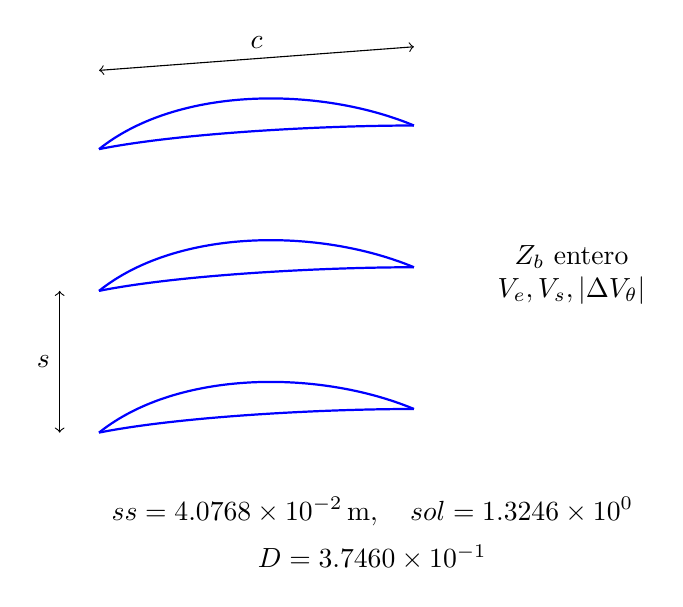
\begin{tikzpicture}\foreach \y in {0,1.8,3.6}{\draw[blue,thick] (0,\y) .. controls (1,\y+.8) and (2.8,\y+.8) .. (4,\y+.3);\draw[blue,thick] (0,\y) .. controls (1,\y+.2) and (2.8,\y+.3) .. (4,\y+.3);}\draw[<->] (-.5,0)--(-.5,1.8) node[midway,left] {$s$};\draw[<->] (0,4.6)--(4,4.9) node[midway,above] {$c$};\node[align=center] at (6,2) {$Z_b$ entero\\$V_e,V_s,|\Delta V_\theta|$};\node[below,align=center] at (3.5,-0.7) {$ss=4.0768\times10^{-2}\,\mathrm{m},\quad sol=1.3246\times10^{0}\,$};\node[below,align=center] at (3.5,-1.2999999999999998) {$D=3.7460\times10^{-1}\,$};\end{tikzpicture}\end{center}\end{document}